\subsection{Quadratmeterpreise}
Ein weiterer wichtiger Aspekt für ein realistisches Portfolio sind die Quadratmeterpreise. Die ungleiche Verteilung der Quadratmeterpreise ist allgemein bekannt. München gilt als die kostspieligste Stadt in Deutschland und im Bundesland Bayern. Gemäß dem Bericht zum Immobilienmarkt liegen die Quadratmeterpreise für Eigenheime in der Stadt und im Landkreis München bei einem durchschnittlichen Preis von 10.200 EUR. In Kronach liegen die Preise bei 1.300 EUR \parencite{bayernlabo2024}. Es gibt große Varianz in den Preisen. Daher müssen die Darlehenspunkte an die jeweiligen Quadratmeterpreise des Standorts angeglichen werden. In Abbildung \ref{fig:preis} sind die Angebotspreise für Eigenheime in den bayerischen Landkreisen und kreisfreien Städten pro Quadratmeter in Euro dargestellt. Die Quadratmeterpreise für das Jahr 2023 wurden aufgeführt.
\begin{figure}[htbp]
    \centering
    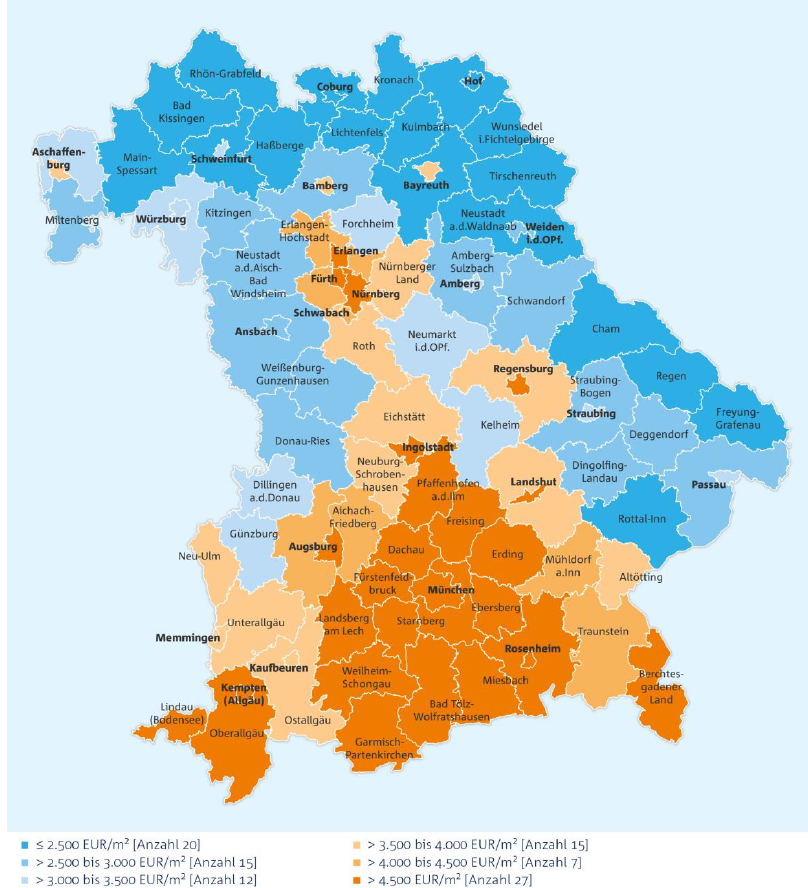
\includegraphics[width=0.8\textwidth]{figures/preism2.png}
    \caption{Angebotspreise 2023 in den bayerischen Landkreisen und kreisfreien Städten – Eigenheime – in EUR/m². Quelle: empirica-Preisdatenbank (Basis: VALUE Marktdaten) }
    \label{fig:preis}
\end{figure}
\FloatBarrier